\documentclass{beamer}

\usepackage{pgf}  
\usepackage{tikz}
\usetikzlibrary{arrows}
\usepgflibrary{shapes.arrows} 
\usetikzlibrary{intersections}
\usetikzlibrary{calc}
\usetikzlibrary{fit}
\usetikzlibrary{automata,positioning}
\usepackage{pgfplots,stackengine}
\usepackage{fontspec}
\usepackage{fancyvrb}
\usepackage{wasysym}
\usepackage{unicode-math}
\usepackage{import}
\usepackage{rotating}
\usepackage{gensymb}
\usepackage{chemfig}
\usepackage{rotating}
\usepackage{booktabs}
\usepackage{pifont}
\usepackage{wrapfig}
\usepackage{mathtools}
\usepackage{graphbox}
\usepackage[absolute,overlay]{textpos}
\usepackage[euler-digits,euler-hat-accent]{eulervm}
%\logo{\pgfputat{\pgfxy(.45,.5)}{\pgfbox[center]{\includegraphics[width=1.7cm]{Figures/Bioclipse.png}}}}

\usetheme{Copenhagen}
\usecolortheme{beaver}

\setbeamercolor{block title}{use=structure,fg=white,bg=red!75!black}
\setbeamercolor*{item}{fg=red}

\newcommand{\unilogo}{
  \setlength{\TPHorizModule}{1pt}
  \setlength{\TPVertModule}{1pt}
   % textblock{}{x,y}: pos(x) = leftUpperCorner + (x * \TPHorizModule), pos(y) = leftUpperCorner - (y * \TPVertModule)
  \begin{textblock}{1}(0,0)
   
\includegraphics[height=27pt, align=c]{Figures/uu.png}\hspace*{10pt}
\includegraphics[height=9pt, align=c]{Figures/ORN.png}
  \end{textblock}
  } 

\pgfmathdeclarefunction{gauss}{2}{%
  \pgfmathparse{1/(#2*sqrt(2*pi))*exp(-((x-#1)^2)/(2*#2^2))}%
}
  
\makeatletter
    \newcases{mycases}{\quad}{%
        \hfil$\m@th\displaystyle{##}$}{$\m@th\displaystyle{##}$\hfil}{\lbrace}{.}
\makeatother

\addtobeamertemplate{frametitle}{}{%
    \unilogo
}

\begin{document}
\graphicspath{{Figures/}}
\setsansfont[ItalicFont = Optima Italic,
             BoldFont = Optima Bold,
             Ligatures=TeX ]
            {Optima Regular}
\setmainfont[ItalicFont = Optima Italic,
             BoldFont = Optima Bold,
             Ligatures=TeX]
            {Optima Regular}
\newfontfamily\comment[]{Chalkboard}
\newfontfamily\zA[Ligatures={Common, Rare}, Variant=1] {Zapfino}
\newfontfamily\zB[Ligatures={Common, Rare}, Variant=2] {Zapfino}
\newfontfamily\zC[Ligatures={Common, Rare}, Variant=3] {Zapfino}
\newfontfamily\zD[Ligatures={Common, Rare}, Variant=4] {Zapfino}
\newfontfamily\zE[Ligatures={Common, Rare}, Variant=5] {Zapfino}
\newfontfamily\zF[Ligatures={Common, Rare}, Variant=6] {Zapfino}
\newfontfamily\zG[Ligatures={Common, Rare}, Variant=7] {Zapfino}

\title{Conformal prediction and Venn-ABERS prediction using CPSign}   
\author{Jonathan Alvarsson} 
\titlegraphic{\vfill
\includegraphics[width=18em]{Figures/ORN_large.png}}
\date{October 2019} 

\setbeamertemplate{background}{%
    \parbox[c][\paperheight]{\paperwidth}{%
        \vfill
        \hfill
        
\includegraphics[height=0.65\textheight]{Figures/sigill.png}
    }   
}
\frame{\unilogo\titlepage} 
\setbeamertemplate{background}{}

\section{Conformal prediction}
    \begin{frame}
    \frametitle{Outline}
    \begin{minipage}{0.25\textwidth}
    \mbox{}
    \end{minipage}
    \begin{minipage}{0.6\textwidth}
    \tableofcontents
    \end{minipage}
    \end{frame}
    
\subsection{Predict with confidence}
    \frame{
        \frametitle{Predict with confidence}
        \framesubtitle{Know how sure you are about each individual prediction}
        \begin{block}{Current case in QSAR}
        Commonly in QSAR we estimate the performance of a model using a \alert{test set} (or cross validation).
        
        \vspace{1\baselineskip}

        But when we make a prediction there is always the suspicion that the
        molecule that we are making a prediction for might be too different
        from the test set and then the question arise: \alert{Can we trust this
        particular prediction?}
        
        \vspace{1\baselineskip}

        (One approach to this is based on the applicability domain concept)
        \end{block}
    }
    
    \frame{
        \frametitle{Predict with confidence}
        \framesubtitle{Know how sure you are about each individual prediction}
        \begin{block}{Conformal prediction}
            (\textit{We will look only at classification today}) \\

            With conformal prediction we are instead predicting \alert{one
            rank score (p-values) for each class} indicating whether the molecule is of
            that class.
        \end{block}
    }

\subsection{Mondrian}
    \frame{
        \frametitle{Mondrian method}
        \framesubtitle{The classes are treated separately}
        \begin{block}{Mondrian method}
            We are modelling each class separately and get two
            independent predictions --- one for each class (They \alert{don't sum up
            to 1})
        \end{block}
        \hfill
        \begin{minipage}{0.45\textwidth}
            \small
            \begin{block}{Pros}
                \begin{itemize}
                    \item We get a \alert{confidence score for each prediction}
                    \item We are \alert{not sensitive to unbalanced data sets}
                \end{itemize}
            \end{block}
        \end{minipage}
        \hfill
        \begin{minipage}{0.45\textwidth}
            \small
            \begin{block}{Cons}
                \begin{itemize}
                    \item We \alert{can't calculate common performance measures} like, \textit{e.g.}, area under ROC curve (AUROC).
                    \item People are not used to this
                \end{itemize}
            \end{block}
        \end{minipage}
        \hfill
    }

% define a command for drawing the horizontal lines
% optional argument: add options to the node
% 1st mandatory argument: y-value of the horizontal line
% 2nd mandatory argument: confidence number
\NewDocumentCommand\HLine{O{}mm}{
    \draw [red,dashed]
    ({rel axis cs:0,0} |- {axis cs:0,#2}) --
    node [font=\footnotesize,below,#1] {confidence=#3}
    ({rel axis cs:1,0} |- {axis cs:0,#2});
}

\frame{
        \frametitle{Mondrian method}
        \framesubtitle{Let's look at an example}

        \begin{block}{An example, classification (\texttt{A} or \texttt{N}?)}
        \centering
        \begin{tikzpicture}[baseline=(current bounding box.center), scale=0.8]
            \begin{axis}[
                % only show ticks at x values that are used ...
                xtick=data,
                % ... and assign these labels to them
                xticklabels={
                    $p$[\texttt{A}]=0.137,
                    $p$[\texttt{N}]=0.488,
                },
                axis x line*=bottom,
                axis y line=left,
                enlarge x limits=0.2,
                ytick={0.15, 0.30, 0.45},
                ylabel=$p$-value,
                x=3.5cm,
                ymin=0,
                ymax=0.55,
                bar width=0.7cm,
                xtick style={draw=none},
            ]
                \addplot[ybar, black,fill=black!30!white] coordinates {
                    % replaced the symbolic coords with numbers
                    (0, 0.137)
                    (1, 0.488)
                };

                % use the above definition to add the horizontal lines
                \HLine{0.50}{0.50}
                \HLine[above]{0.14}{0.86}
                \HLine{0.13}{0.87}
            \end{axis}
        \end{tikzpicture}
        \begin{minipage}{0.45\textwidth}
        \scriptsize
        \begin{tabular}{ccc}
        \toprule
        Confidence & p-value & Prediction \\
        \midrule
        0.5  & 0.5  &\{\O\} \\
        0.86 & 0.14 &\{\texttt{N}\} \\
        0.87 & 0.13 &\{\texttt{A, \kern -5pt N}\} \\
        \bottomrule
        \end{tabular}
        \end{minipage}
        \end{block}
    }

\section{Hands-on}
    \subsection{What you might want to know}
    \frame{
        \frametitle{What you might want to know}
        \framesubtitle{Some info regarding our predictions}
        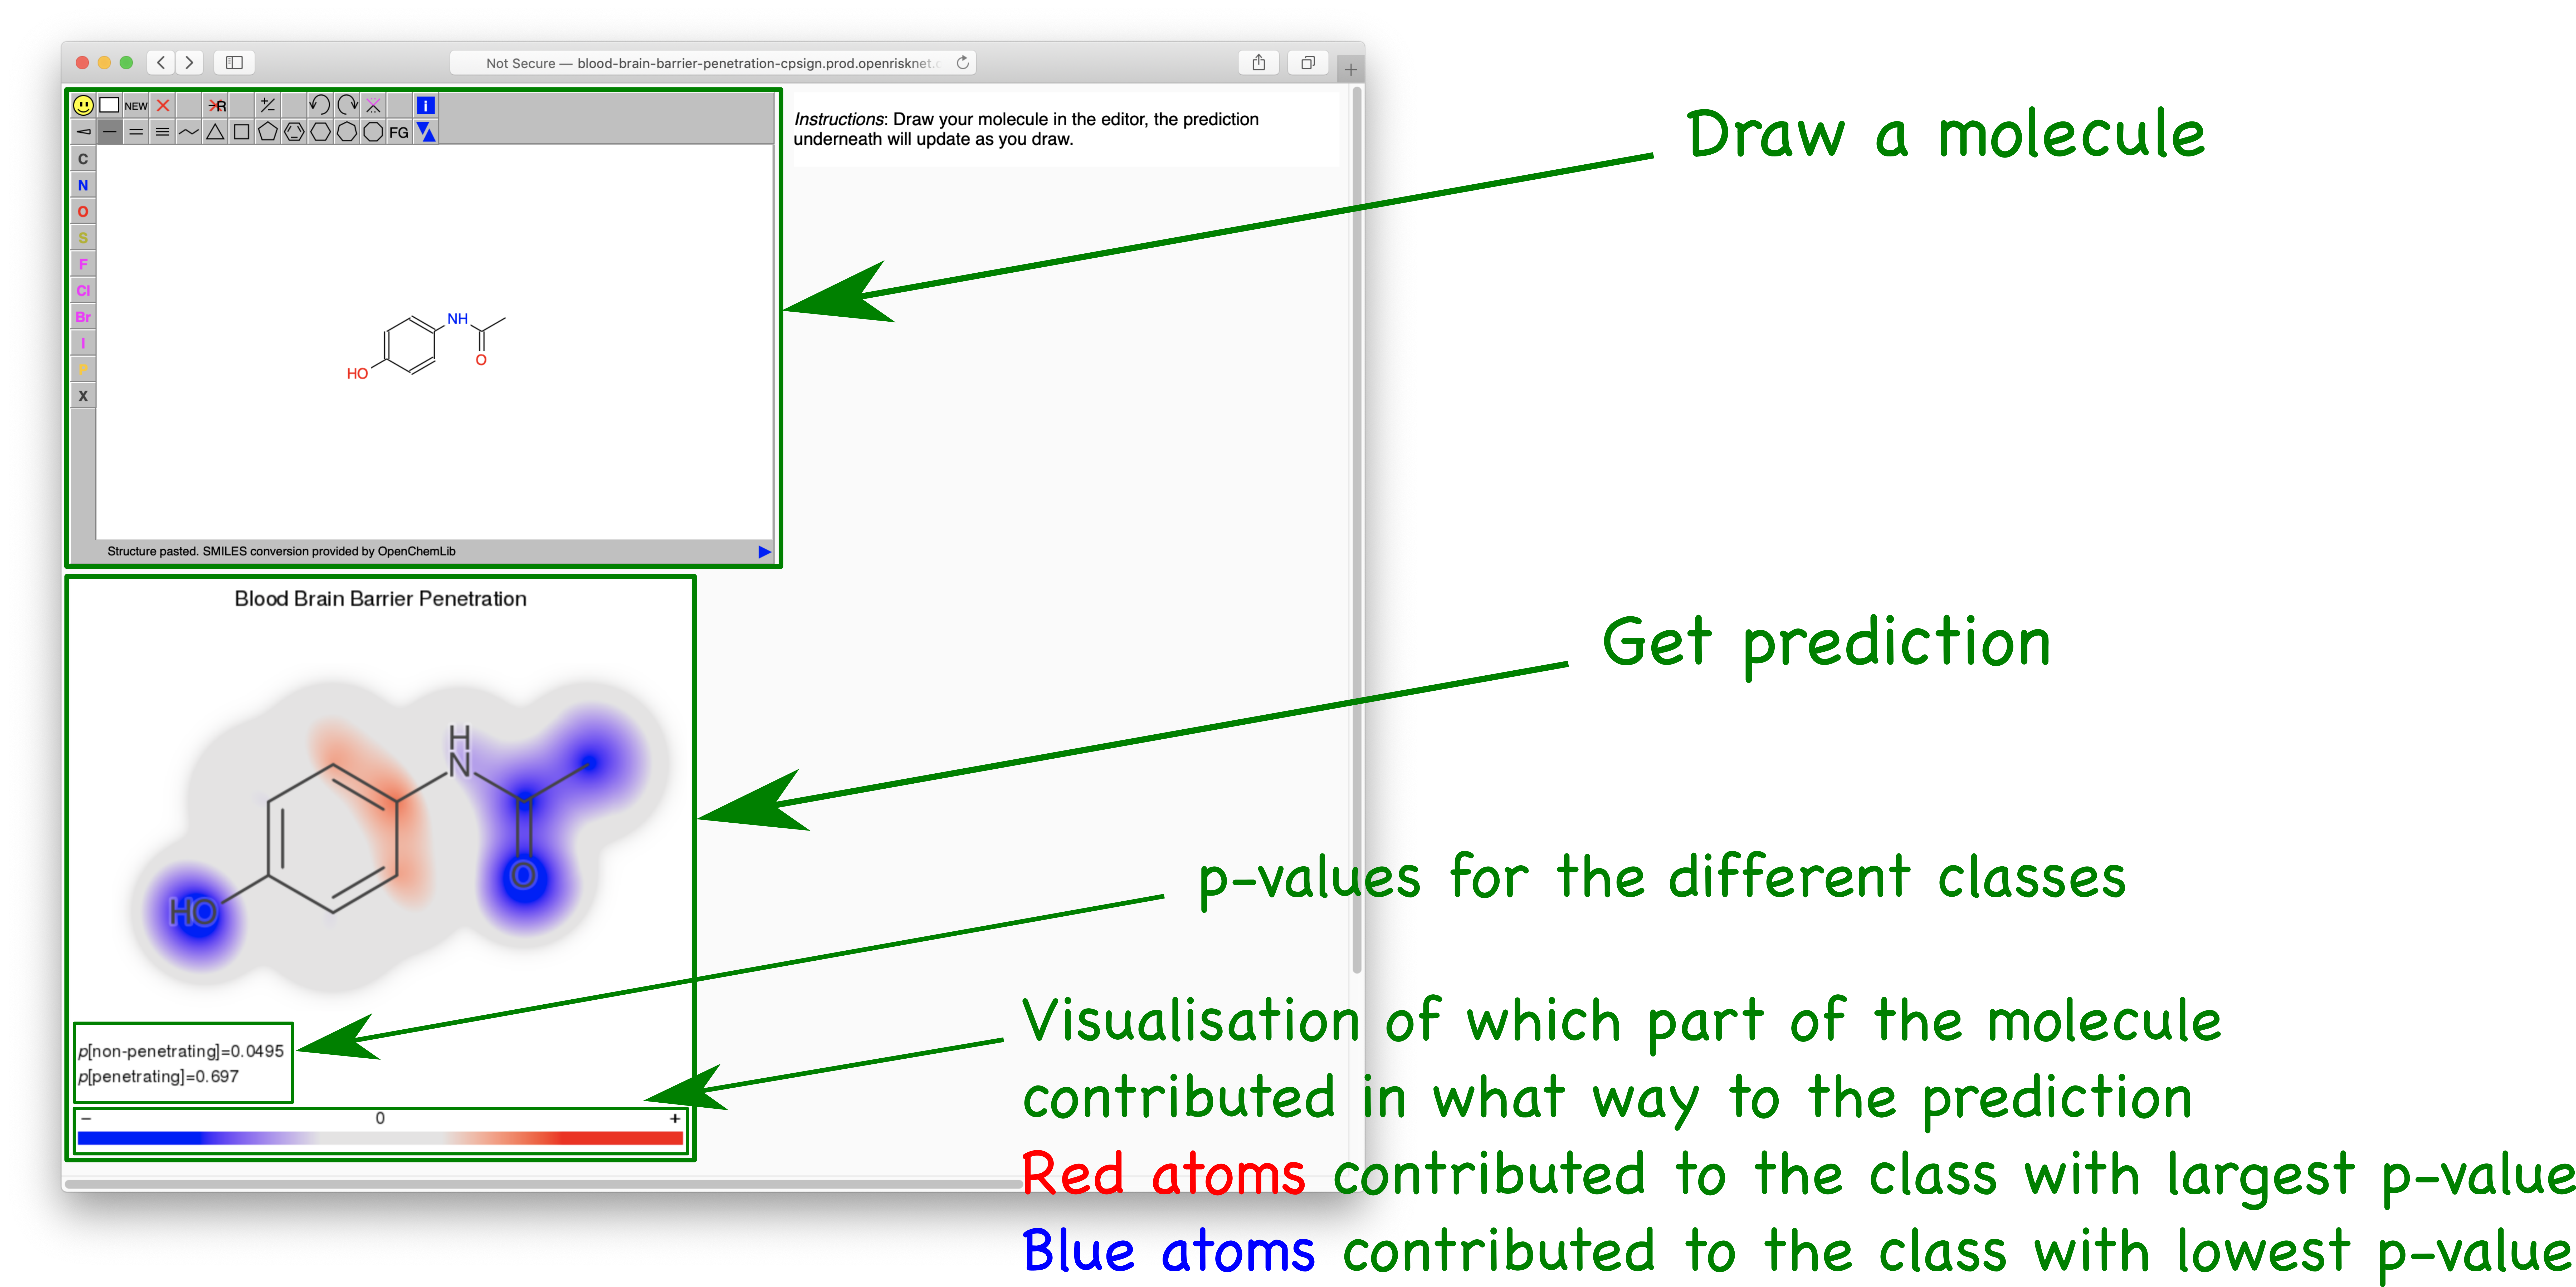
\includegraphics[width=1\textwidth]{Figures/serviceImage.png}
    }
    
    \subsection{Let's get hands-on!}
    \frame{
        \frametitle{Let's get hands-on!}
        \framesubtitle{A chance to try it out a bit!}
        \url{http://blood-brain-barrier-penetration-cpsign.prod.openrisknet.org/draw/}
    }

\section{Venn-ABERS prediction}

    \subsection{The consensus modelling}
    \frame{
        \frametitle{The consensus modelling}
        \framesubtitle{}
        \begin{block}{Consensus modelling}
        We have seen a number of prediction models now and it was suggested
        that we would use them together in a consensus approach.  
        \end{block}
    }
    \frame{
        \frametitle{The consensus modelling}
        \framesubtitle{Trouble}
        \begin{block}{Trouble}
        {\centering Conformal prediction is Mondrian \\ $\Rightarrow$ \\ The p-values does not sum up to 1\\}
        
        \vspace{1\baselineskip}
        The consensus approach could not handle the p-values from our conformal
        prediction approach.
        \end{block}
    }
    \subsection{Non-Mondrian}
    \frame{
        \frametitle{Non-Mondrian}
        \framesubtitle{Venn-ABERS produces probabilities}
        \begin{block}{Non-Mondrian method}
            Venn-ABERS prediction is a more ``classic'' approach, \textit{i.e.}, non-Mondrian. 
        \end{block}
        \hfill
        \begin{minipage}{0.45\textwidth}
            \small
            \begin{block}{Pros}
                \begin{itemize}
                    \item We get a predicted \alert{probability for each class}
                    \item We \alert{can calculate common performance measures} like, \textit{e.g.}, AUROC.
                \end{itemize}
            \end{block}
        \end{minipage}
        \hfill
        \begin{minipage}{0.45\textwidth}
            \small
            \begin{block}{Cons}
                \begin{itemize}
                    \item We are \alert{sensitive to unbalanced data sets}.
                \end{itemize}
            \end{block}
        \end{minipage}
        \hfill

    }
    \setbeamertemplate{background}{%
        \parbox[c][\paperheight]{\paperwidth}{%
            \vskip -14 ex \hskip -5 em
            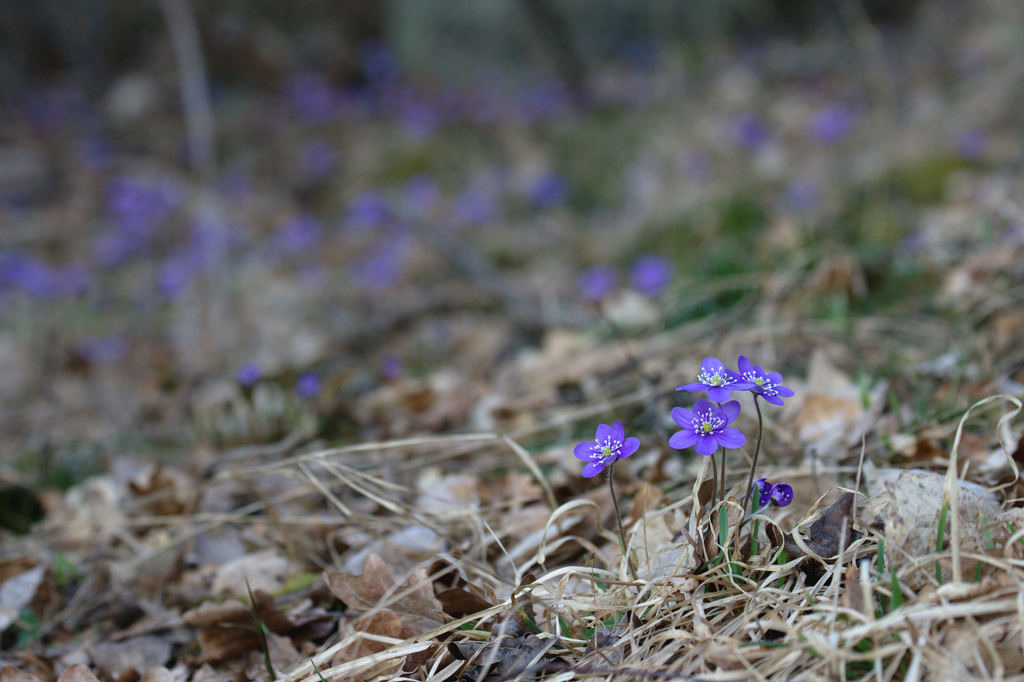
\includegraphics[height=1.275\paperheight]{Figures/blasippa.jpg}
        }   
    }
    \begin{frame}[plain]
        \vfill{\Huge\qquad\color{white} \zB Thank \zC you}\vfill
    \end{frame}
    \setbeamertemplate{background}{}
\end{document}
